\documentclass[convert={density=300,size=1080x800,outext=.png}]{standalone}
\usepackage{tkz-graph}
\usetikzlibrary{arrows,positioning,shapes,shapes.multipart,patterns,mindmap,shadows}
\usepackage{xcolor}
\usepackage{helvet}

\renewcommand{\familydefault}{\sfdefault}

\definecolor{blue}{RGB}{4, 83, 156}  % hex: #04539C
\definecolor{gray}{RGB}{148, 147, 132}  % hex: #8A9384
\definecolor{yellow}{RGB}{251, 187, 6}  % hex: #FBBB06

\begin{document}

\begin{tiny}
    \resizebox{10cm}{!}{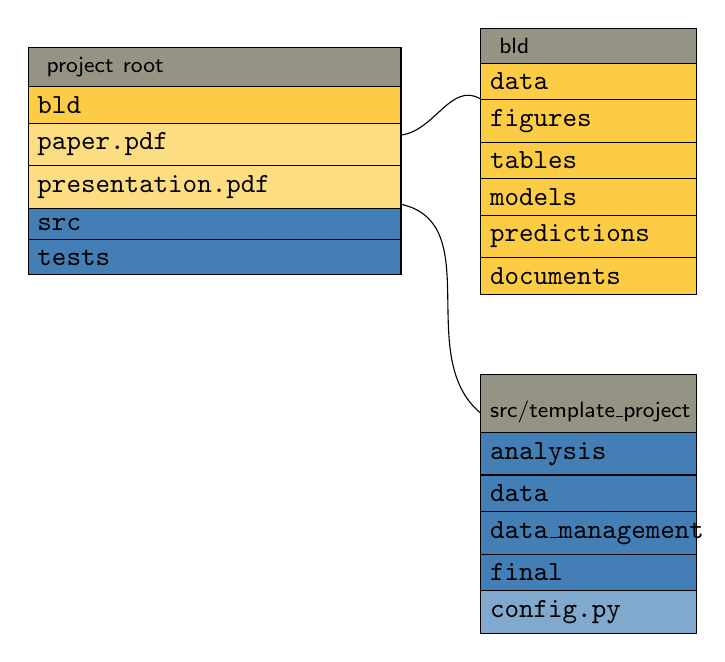
\begin{tikzpicture}[node distance=1cm, auto]
            \node (1) [
                rectangle split,
                rectangle split parts=6,
                rectangle split part fill={
                        gray,
                        yellow!75,
                        yellow!50,
                        yellow!50,
                        blue!75,
                        blue!75,
                    },
                draw,
                text width=4.50cm
            ]
            {
                \nodepart{one}
                \begin{footnotesize}
                    project root
                \end{footnotesize}
                \nodepart{two}
                \texttt{bld}
                \nodepart{three}
                \texttt{paper.pdf}
                \nodepart{four}
                \texttt{presentation.pdf}
                \nodepart{five}
                \texttt{src}
                \nodepart{six}
                \texttt{tests}
            };

            \node (2) [
                rectangle split,
                rectangle split parts=7,
                rectangle split part fill={
                        gray,
                        yellow!75,
                        yellow!75,
                        yellow!75,
                        yellow!75,
                        yellow!75,
                        yellow!75,
                    },
                draw,
                text width=2.50cm,
                right=of 1
            ]
            {
                \nodepart{one}
                \begin{footnotesize}
                    bld
                \end{footnotesize}
                \nodepart{two}
                \texttt{data}
                \nodepart{three}
                \texttt{figures}
                \nodepart{four}
                \texttt{tables}
                \nodepart{five}
                \texttt{models}
                \nodepart{six}
                \texttt{predictions}
                \nodepart{seven}
                \texttt{documents}
            };

            \node (3) [
                rectangle split,
                rectangle split parts=6,
                rectangle split part fill={
                        gray,
                        blue!75,
                        blue!75,
                        blue!75,
                        blue!75,
                        blue!50,
                    },
                draw,
                text width=2.50cm,
                below=of 2
            ]
            {
                \nodepart{one}
                \begin{footnotesize}
                    src/template\_project
                \end{footnotesize}
                \nodepart{two}
                \texttt{analysis}
                \nodepart{three}
                \texttt{data}
                \nodepart{four}
                \texttt{data\_management}
                \nodepart{five}
                \texttt{final}
                \nodepart{six}
                \texttt{config.py}
            };

            \draw[-, out=8, in=150] (1) to (2);
            \draw[-, out=-13, in=140] (1) to (3);
        \end{tikzpicture}}
\end{tiny}

\end{document}
